\documentclass[12pt,oneside,smallheadings,chapterprefix=true]{article}
\usepackage[extendedchars]{grffile}

\usepackage{amsmath} %Never write a paper without using amsmath for its many new commands
\usepackage{amssymb} %Some extra symbols
\usepackage{setspace}
\usepackage{paralist}
%\usepackage{a4wide}
\usepackage[a4paper,left=2.54cm, right=2.54cm, top=2.54cm, bottom=2.54cm, footskip=0.5cm]{geometry}		% footskip = Abstand zwischen Fußnote und Text
\usepackage{ctable}
\usepackage{lscape}	% Querformat
\usepackage{graphicx}
\graphicspath{{./Figures/}}
\usepackage[sort&compress]{natbib}
\usepackage{caption}
\usepackage[none]{hyphenat} % keine Silbentrennung
\usepackage{appendix}
%\usepackage[ansinew]{inputenc}
%\usepackage{subfigure}
\usepackage[parfill]{parskip}
\usepackage[pdftex]{hyperref}
%\hypersetup{bookmarks=true, unicode=true, colorlinks=true, linkcolor=black, citecolor=black, filecolor=black,  urlcolor=black} % lesbar machen
\usepackage{helvet}
\usepackage{eurosym}
\usepackage{dcolumn} % for tables
\usepackage{dcolumn}
\usepackage{longtable}
\usepackage{setspace}
\usepackage{float}
\usepackage{url}
\usepackage{color}
\usepackage{tabularx}
%\usepackage{subfig}
\usepackage{subcaption}
\usepackage[section]{placeins}

\usepackage[utf8]{inputenc}
\usepackage{fourier} 
\usepackage{array}
\usepackage{makecell}
\usepackage{lscape}


\renewcommand\theadalign{bc}
\renewcommand\theadfont{\bfseries}
\renewcommand\theadgape{\Gape[2pt]}
\renewcommand\cellgape{\Gape[2pt]}
\renewcommand{\cellalign}{tl}
\renewcommand{\theadalign}{cl}


\newcommand{\note}[1]{\footnote{\begin{doublespace}#1\end{doublespace}}}
 
\newcommand{\arrayfontsize}{\fontsize{7}{7}\selectfont}
\interfootnotelinepenalty=10000


\begin{document}

%\tableofcontents

\setlength{\textwidth}{14.0cm}

\onehalfspacing

\vspace*{0.7cm}
\begin{center}
\begin{huge}
Public support for global vaccine sharing in the COVID-19 pandemic\footnote{Research for this contribution is part of the Cluster of Excellence "Contestations of the Liberal Script" (EXC 2055, Project-ID: 390715649), funded by the Deutsche Forschungsgemeinschaft (DFG, German Research Foundation) under Germany´s Excellence Strategy.}
\end{huge}
\end{center}

\vspace*{0.5cm}

\begin{center}
Heike Klüver, Humboldt-Universität zu Berlin \\
Felix Hartmann, Humboldt-Universität zu Berlin \\ 
Macartan Humphreys, WZB Berlin Social Science Center/Columbia University \\
Ferdinand Geissler, Humboldt-Universität zu Berlin \\
Johannes Giesecke, Humboldt-Universität zu Berlin



\end{center}		
		
		
		\vspace*{1cm}
										
								

\singlespacing
\begin{sloppypar}
	\textbf{Abstract:} 
Even though the COVID-19 pandemic can only be overcome if enough people are vaccinated worldwide, the global distribution of the vaccines is extremely unequal. While only 0.3\% of people in low-income countries are fully vaccinated, as much as 43.7\% of the population in high-income countries have already been fully vaccinated. Given that governments need to secure public support for sharing vaccines with poorer countries instead of administering a third booster vaccination to their own people, it is important to understand what drives mass support for vaccine sharing. Building on a 


 and to identify ways through which governments can increase solidarity with other countries in need. 


\end{sloppypar}






\thispagestyle{empty}

\newpage
\doublespacing

\setcounter{page}{1}

\section*{Introduction}
Vaccination is the key to overcome the COVID-19 pandemic. A number of vaccines have been developed in record time and 4.36 billion doses have been administered globally  until today. However, the global distribution of the vaccines is extremely unequal. While only 0.3\% of people in low-income countries are fully vaccinated, as much as 43.7\% of the population in high-income countries are fully vaccinated.\footnote{Source: https://github.com/favstats/vacccprogress} Vaccine inequity is not only a humanitarian disaster, but it also makes it impossible to reach global herd immunity to sustainably stop the spread of the virus. It has been estimated that  approximately 70\% of the worldwide population must be fully vaccinated to end the COVID-19 pandemic \citep{Randolph2020}. The delta variant has pushed the threshold for global herd immunity to  80\% and potentially approaching 90\%, according to the Infectious Diseases Society of America.\footnote{Source:  https://fortune.com/2021/08/04/delta-variant-herd-immunity-higher-threshold/} Despite the importance of globally distributing COVID-19 vaccines to stop the pandemic, a number of Western countries are launching campaigns for a third booster vaccination or even dump vaccines as demand slowed down \citep{Mahase2021}. Hence,  vaccines against COVID-19 will continue to be scarce  and poorer countries will struggle obtaining  sufficient vaccines for their citizens in the foreseeable future. On 4 August 2021, WHO director Tedros Adhanom Ghebreyesus therefore called for a moratorium halting COVID-19 vaccine boosters in favor of unvaccinated.\footnote{Source: https://www.reuters.com/business/healthcare-pharmaceuticals/who-calls-moratorium-covid-19-vaccine-booster-doses-until-september-end-2021-08-04/} Given that governments need to secure public support for sharing vaccines with poorer countries instead of administering a third dose to their own people, it is crucially important to understand the determinants of citizen preferences for global vaccine sharing and to identify ways through which governments can increase solidarity with other countries in need. 

While previous research has focused on mapping the international distribution of COVID-19 vaccines (CITATIONS), little is known about public preferences for global vaccine sharing. Building on previous work on European solidarity during the Eurozone crisis \citep{Bechtel2017,Kuhn2018,Kuhn2020,Stoeckel2018} and preferences for international climate agreements \citep{Bechtel2013,Bechtel2017,Bechtel2019},  
we argue that popular preferences for global vaccine sharing are based on a cost-benefit calculation and shaped by the specific costs and benefits for the donor country and the participation of other countries. We moreover argue that public support can be increased through information campaigns appealing to the self-interest of citizens. We test our theoretical expectations on the basis of a randomized intervention and a conjoint experiment that were fielded in a representative online survey among 13,782 citizens in Germany at the beginning of the vaccination roll-out. 

The results of our study have major implications for the current public debate on global vaccine distribution, but also for international solidarity and international cooperation more generally. On the one hand, the COVID-19 vaccination is a highly salient issue for all citizens worldwide which provides a unique opportunity to study popular preferences for globally sharing scarce goods. On the other hand, since herd immunity is a global public good as the pandemic can only be overcome if all countries worldwide are immunized, our findings can furthermore inform the literature on preferences for international cooperation. 



%%%%%%%%%%%%%%%%%%%%%%%%%%%%%%%%%%%%%%%%%%%%%
%%%%%%%%%%%%%%%%%%%%%%%%%%%%%%%%%%%%%%%%%%%%%

\section*{Design}
\label{sec:design}

We have conducted an experimental study which was fielded as an online survey among 13,782 citizens in Germany from 29 April to 10 May 2021. Our population of interest consists of all German citizens between 18 and 75. We rely on a representative sample which was drawn with the help of the online-access panel provider \hspace{0pt}Respondi\hspace{0pt}\hspace{0pt}. All analyses were prespecified in a preregistered analysis plan made available at the Center for Open Science (https://osf.io/69mpy) and the study obtained IRB approval at Humboldt-Universität zu Berlin.
  
During the field time of the survey, only 7.7 (29 April) to 9.7 (10 May) per cent of the population was fully vaccinated while 19 (29 April) to 24 (10 May) per cent received the first dose.\footnote{Source: https://ourworldindata.org/covid-vaccinations} At the same time, 77 per cent of the respondents indicated that they either were already vaccinated (33 per cent), that they definitely want to get vaccinated against COVID-19 (44 per cent) or that they were undecided (11 per cent). Hence, at the time when we conducted the experimental study, COVID vaccines were an extremely scarce good as public demand greatly exceeded the supply with vaccines. 

The experimental study relies on a randomized intervention followed by a Conjoint experiment. In the first experiment, participants were randomly assigned to a \emph{treatment group} which is exposed to a video explaining the benefits of global vaccine sharing and a \emph{control group} which did not see a video. Subsequently respondents were questioned whether they support the international distribution of vaccines (attitudinal outcome) and were offered the opportunity to donate money to UNICEF which was put in charge for global vaccine sharing (behavioural outcome). More specifically, respondents earned 75 so-called "`Mingle Points"' cents for their participation in the survey which corresponds to 0,75 Euros. We offered them  50 additional Mingle Points and gave them the following choice. They could either keep the 50 Mingle Points for themselves yourself or donate all or part of them to UNICEF for the worldwide distribution of corona vaccines. For every point they donated, we donated 1.5 Euro Mingle points to UNICEF (see table \ref{table:mingle} in the Supplementary Materials).

Afterwards, all respondents were included in a Conjoint experiment in which respondents two hypothetical proposals about Germany's contribution to global vaccine sharing. Respondents were asked  to indicate which proposal they would prefer and to rate each proposal with regard to how likely they would vote in favor of or against it in a referendum. The Conjoint experiment allows for estimating the effect of each factor on respondents' preferences for global vaccine sharing. We randomize the following dimensions: contribution to global vaccine sharing, contribution to global vaccine sharing relative to other countries, number of countries participating in global vaccine sharing, economic benefits and health benefits. The factors were assigned with independent probabilities. Each respondent received three vignettes successively. However, respondents did not see that same profile twice. 

Before both experiments, we collected a number of covariates that to examine to what extent international vaccine solidarity is moderated by individual attitudes and attributes. We included trust in government and local health system (Mesch
\& Schwirian, 2015), economic hardship and education (Bertoncello et al.,
2020), minority group status and maternal age (Danis et al., 2010), risk
perception (Brewer et al., 2007) and health status (Guay et al., 2019).
Additionally, we collect data on political attitudes, attitudes towards
migrants, and attitudes towards COVID-19 as well as indicators that
identify groups who are eligible for the vaccine.\footnote{Please see the
questionnaire in the Supplementary Materials for more details.}


%%%%%%%%%%%%%%%%%%%%%%%%%%%%%%%%%%%%%%%%%%%%%
%%%%%%%%%%%%%%%%%%%%%%%%%%%%%%%%%%%%%%%%%%%%%

\section*{Results}
\label{sec:results}

Figure \ref{fig:conjoint_choice} reports the results of the Conjoint experiment. The results are largely in line with our theoretical expectations. First, the number of vaccine doses that Germany would distribute to other countries negatively affects solidarity. Thus, citizens are more willing to share a smaller number of vaccine doses with other countries. In other words, international solidarity among citizens decreases with the absolute costs of distribution. Second, we find that it matters for citizens how much other countries are contributing to global vaccine redistribution. Solidarity among citizens is lowest when Germany contributes 20 per cent of all the vaccine doses that are globally shared, but it increases with other countries contributing a higher share to global vaccine sharing. In a similar fashion, we also find that the number of countries that participate in global vaccine sharing positively influences solidarity. Citizens are more willing to donate vaccine doses to poorer countries when more countries participate in global redistribution. With regard to the risk of infection, we show that citizens are more willing to share vaccine doses with poorer countries if these countries constitute a health risk for Germany (e.g. popular tourist destinations or countries with which Germany has strong economic ties). Thus, respondents were more willing to donate vaccine doses to minimize the risk of infections for Germany. 

While all these findings are in line with our theoretical expectations, the result for economic importance is counterintuitive. While we have expected that the economic importance of a country for Germany should increase the willingness of citizens to share vaccine doses, we actually find the opposite effect. The less important a country is to Germany economically, the more willing are citizens to redistribute vaccine doses. Hence, while all the other findings speak for a cost-benefit calculation that fundamentally drive international solidarity among citizens, this finding instead suggests that also the neediness of a country could account for the level of solidarity among citizens. 




\begin{figure}[hbt!]
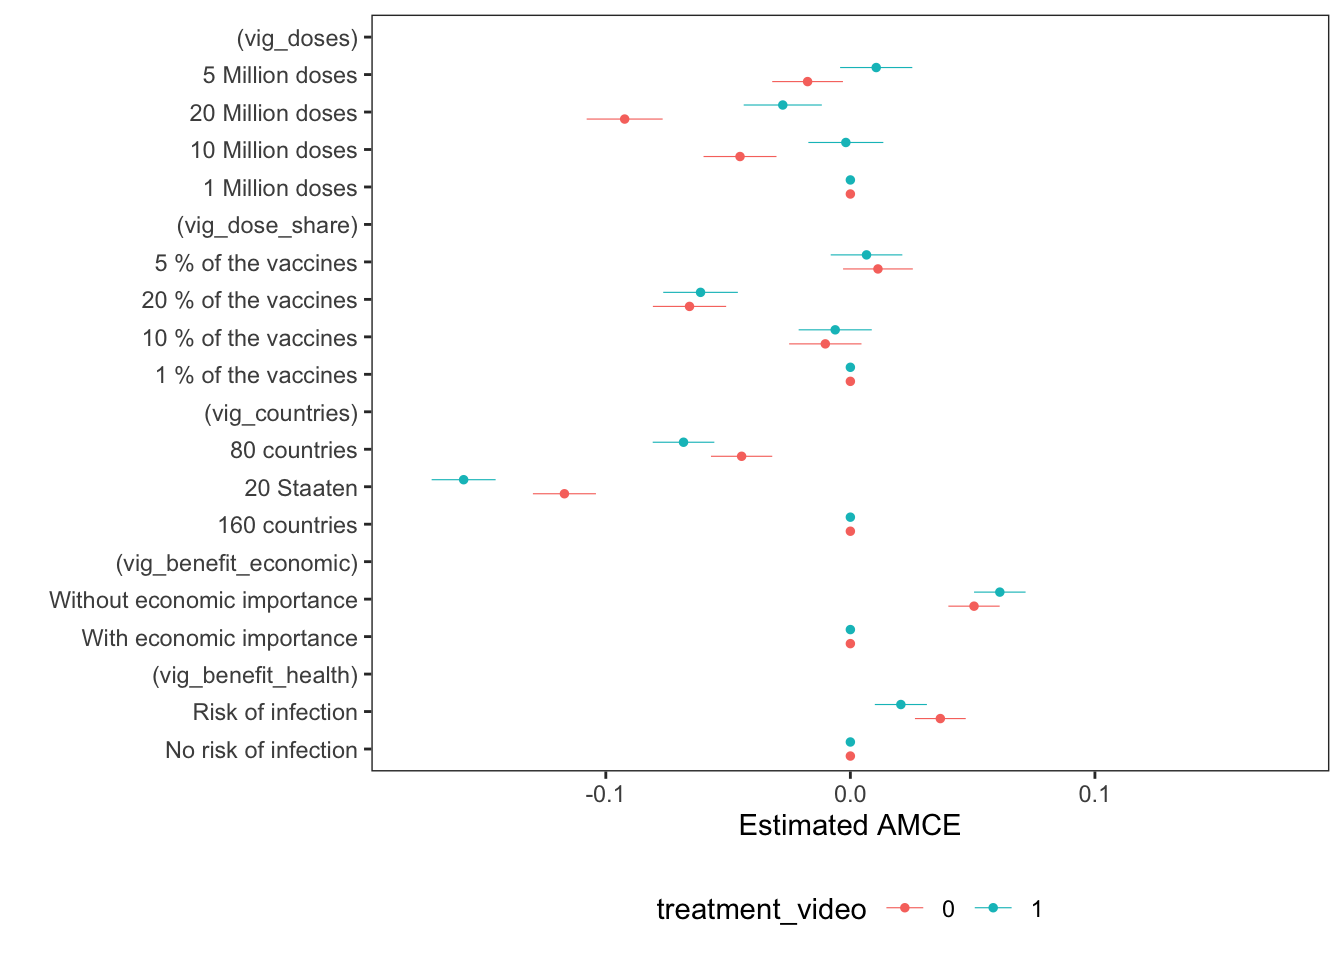
\includegraphics[width=\linewidth]{2_figures/fig_conjoint_choice.png}
\caption{Results of Conjoint Experiments}
\label{fig:conjoint_choice}
%\floatnote{This is a note for this figure.}
\end{figure}



\begin{figure}[hbt!]
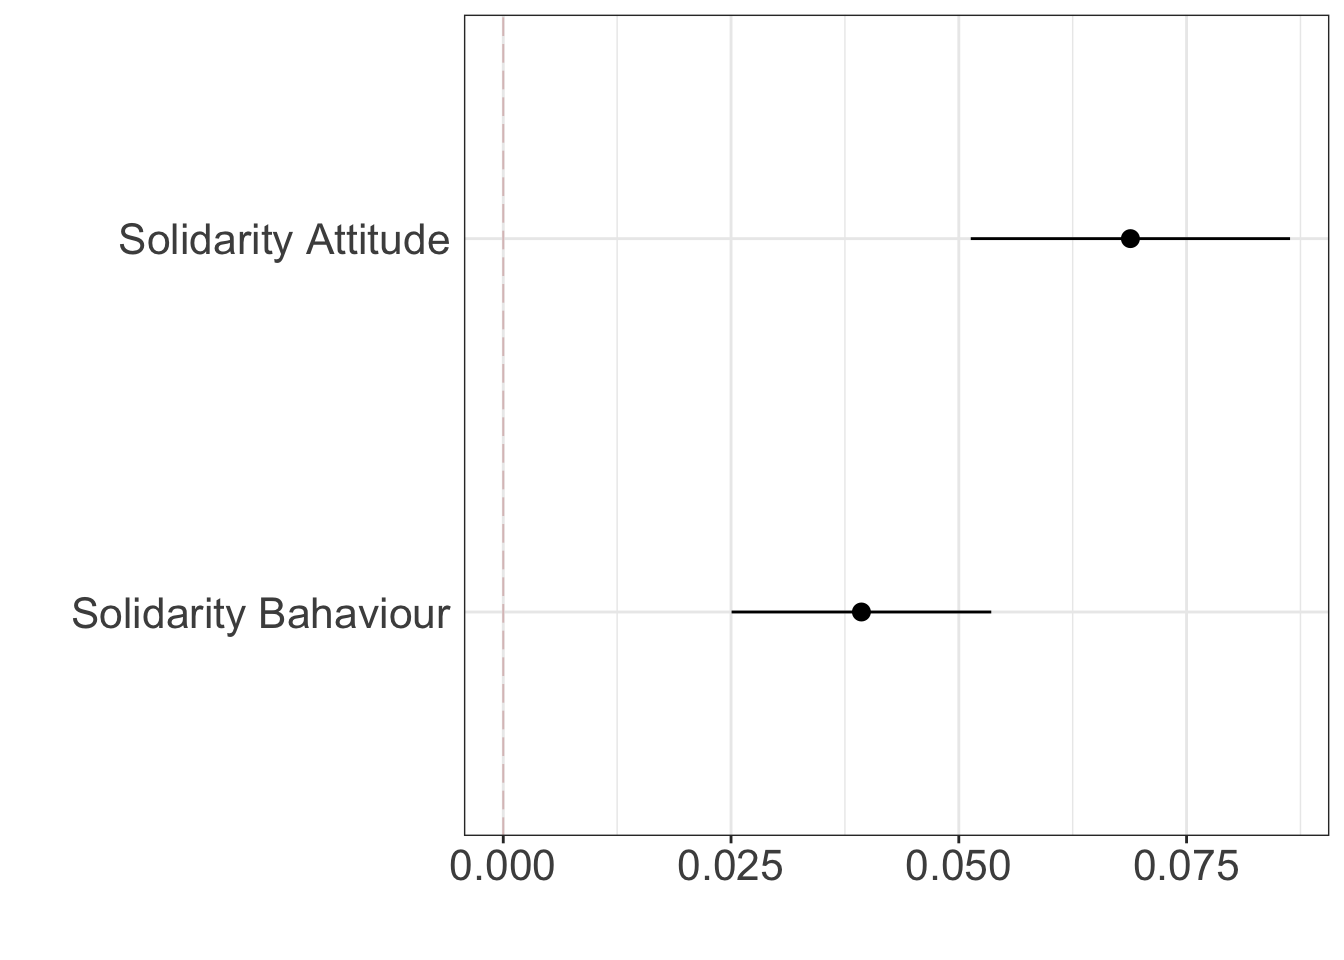
\includegraphics[width=\linewidth]{2_figures/fig_video.png}
\caption{Effect of video treatment on individual solidarity}
\label{fig:video}
%\floatnote{This is a note for this figure.}
\end{figure}


Figure \ref{fig:video} reports the findings of the randomized intervention. We find that respondents in the treatment group which were exposed to the video are significantly more likely to show solidarity both with regard to the attitudinal and the behavioural outcome. More specifically, the willingness to personally support international distribution of vaccines is 0.069 units higher than in the control group. In a similar vein, the donations that respondents made to UNICEF were on average significantly higher in the treatment than in the control group. However, the effect is considerably stronger for the attitudinal than for the behavioural outcome. 




\subsubsection*{Heterogenous Effects} 
We supplement this analysis with a pre-registered machine learning analysis to shed light on how the effects vary by population subgroups.  We use a causal forests approach \citep{wager2018estimation} which is a specific application of the generalized random forests algorithm \citep{athey2019generalized}. We estimate Conditional Average Treatment Effects (CATEs) across all covariates in our data set (for details on covariates, see the Supplementary Materials). The approach randomly partitions the data and identifies which regression trees predict the largest variation in the magnitude of effects (for further details, see the Supplementary Materials). To summarize the results from the causal forests, we calculate a measure of variable 'importance' used to estimate the heterogeneous treatment effects by taking a simple weighted sum of how often a variable was used in a tree split. The results (see Figure 8 in the SM) suggest that the video treatment essentially has a similar affect across all population subgroups. There is only a statistically significant effect for reciprocity attitudes, but this effect is substantially neglible. Thus, information campaigns appealing to self-interest can foster international solidarity among citizens across the board. 


\textcolor{red}{Felix: I am not entirely sure which heterogeneous effects you are precisely looking at. Would be great if you could write this up.} 





%%%%%%%%%%%%%

% HK: This paragraph could be shortened
%Next, we explore how CATE estimates behave when we change a single covariate, while keeping all the other covariates at some fixed value. In Fig. 3 we evaluate a variable of interest across quantiles, while keeping all other covariates at their median. T  We find a negative interaction effect between the high financial and increased freedoms treatment and the \textit{Age} of the respondents. While both treatment show significant effects for younger cohorts, they are less likely to yield significant effects for older subgroups. The possibility to get vaccinated at the local doctor yields slightly stronger predicted treatment effects for the older cohorts in the study. Using the causal forest, we also find evidence that attitudes towards the vaccination explain heterogeneity in the treatment effects. Those respondents who stated that they were \textit{undecided} to get vaccinated showed higher treatment effects for high financial incentives and personal freedoms. Further, increased personal freedoms are predicted to yield higher CATE's for those who show less \textit{solidarity} with others in the society (low values on the scale). The possibility to get vaccinated at the local doctor is more likely to yield treatment effects for those who show more solidarity with others. Lastly, we show that those who do not \textit{support social distancing} once they are vaccinated are also more likely to show strong treatment effects for increased personal freedoms. 






%% Use \bibliography{...} if using BibTeX
\bibliography{solidarity}
\bibliographystyle{apsr}

%TC:subst \printbibliography \bibliography
%TC:macro \field [0,1]
%TC:macro \name [0,0,0,1]
%TC:macro \list [0,0,1]
%% Use \printbibliography if using BibLaTeX
% \printbibliography

\clearpage
%%%%%%%%%%%%%%%%%%%%%%%%%%%%%%%%%%%%%%%%%%%%%%%%%%%%%%% 
\setcounter{page}{1}

\begin{center}
\appendix{\textbf{\Large{Supplementary Materials}}}
\end{center}


%\begin{center}
%\Large{What incentives can spur Covid-19 vaccination uptake?} \\
%\end{center}




%%%%%%%%%%%%%%%%%%%%%%%%%%%%%%%%%%%%%%%
\tableofcontents


\clearpage
\section{Study Design}


\begin{itemize}
\item
  \textbf{Introductory text}: And now we come to the topic of the global
  vaccination campaign. The pandemic can only be defeated if it is
  brought under control globally. In the fight against Covid-19, the
  provision of vaccines is particularly important. The COVAX platform
  was set up under the leadership of the World Health Organization (WHO)
  for the acquisition and fair distribution of vaccines.
\item
  \textbf{Video}: The video can be found here:
  https://www.dw.com/de/impfstoff-f\%C3\%BCr-entwicklungsl\%C3\%A4nder/av-56554104
\end{itemize}

\subsection{Outcome: Willingness to share}


\hypertarget{outcome-personal-donation}{%
\subsection{Outcome: Personal
donation}\label{outcome-personal-donation}}

\begin{itemize}
\item
  \textbf{Personal donation}: You can also contribute to the global
  distribution of the vaccines yourself. UNICEF is working on behalf of
  the COVAX initiative to ensure that the corona vaccines are made
  available to people in the poorest countries.

  Next to the 75 Mingle points that you receive for taking part in this
  survey, you will receive an \textbf{additional 50 Mingle points} from
  us. You can either keep these points yourself or donate all or part of
  them to UNICEF for the worldwide distribution of corona vaccines. For
  every mingle point you donate, we donate 1.5 mingle points to UNICEF.

  Please select how the additional Mingle points should be allocated to
  you or UNICEF.
\end{itemize}




\begin{longtable}[]{@{}lll@{}}
\caption{Bonuses and donations}
\label{table:mingle}
\endfirsthead
\endhead
\toprule
& Your Bonus & Donation to UNICEF\tabularnewline
\midrule
\endhead
1 & 0 Mingle Points & 75 Mingle Points\tabularnewline
2 & 10 Mingle Points & 60 Mingle Punkte\tabularnewline
3 & 20 Mingle Points & 45 Mingle Points\tabularnewline
4 & 30 Mingle Points & 30 Mingle Points\tabularnewline
5 & 40 Mingle Points & 15 Mingle Points\tabularnewline
6 & 50 Mingle Points & 0 Mingle Points\tabularnewline
\bottomrule
\end{longtable}


\begin{itemize}
\tightlist
\item
  \emph{Donations go here:}
  https://www.unicef.de/spenden/jetzt-spenden?purpose=235762
\end{itemize}

    \hypertarget{conjoint-design}{%
\subsection{Conjoint Design}\label{conjoint-design}}

\begin{itemize}
\tightlist
\item
  \textbf{Introductory text}: In the following, we present suggestions
  on how Germany's contribution to the global distribution of vaccine
  doses to poorer countries could look like this year.
\item
  \textbf{Conjoint Design}: Our second outcome measure is a conjoint experiment (two profiles) with randomly assigned factors (uniform) over five attributes. Each respondents will see three pairs. Unit of randomization is respondent pair.
\end{itemize}




\begin{longtable}[]{@{}ll@{}}
\toprule
\begin{minipage}[b]{0.40\columnwidth}\raggedright
\strut
\end{minipage} & \begin{minipage}[b]{0.54\columnwidth}\raggedright
Proposal\strut
\end{minipage}\tabularnewline
\midrule
\endhead
\begin{minipage}[t]{0.40\columnwidth}\raggedright
Sharing of vaccination doses\strut
\end{minipage} & \begin{minipage}[t]{0.54\columnwidth}\raggedright
\{0\} Germany will give away 1 Million doses of its Covid Vaccine\strut
\end{minipage}\tabularnewline
\begin{minipage}[t]{0.40\columnwidth}\raggedright
\strut
\end{minipage} & \begin{minipage}[t]{0.54\columnwidth}\raggedright
\{1\} Germany will give away 5 Million doses of its Covid Vaccine\strut
\end{minipage}\tabularnewline
\begin{minipage}[t]{0.40\columnwidth}\raggedright
\strut
\end{minipage} & \begin{minipage}[t]{0.54\columnwidth}\raggedright
\{2\} Germany will give away 10 Million doses of its Covid Vaccine\strut
\end{minipage}\tabularnewline
\begin{minipage}[t]{0.40\columnwidth}\raggedright
\strut
\end{minipage} & \begin{minipage}[t]{0.54\columnwidth}\raggedright
\{3\} Germany will give away 20 Million doses of its Covid Vaccine\strut
\end{minipage}\tabularnewline
\begin{minipage}[t]{0.40\columnwidth}\raggedright
Germany's contribution compared to other countries\strut
\end{minipage} & \begin{minipage}[t]{0.54\columnwidth}\raggedright
\{0\} Germany contributes 1\% of the vaccines donated worldwide\strut
\end{minipage}\tabularnewline
\begin{minipage}[t]{0.40\columnwidth}\raggedright
\strut
\end{minipage} & \begin{minipage}[t]{0.54\columnwidth}\raggedright
\{1\} Germany contributes 5\% of the vaccines donated worldwide\strut
\end{minipage}\tabularnewline
\begin{minipage}[t]{0.40\columnwidth}\raggedright
\strut
\end{minipage} & \begin{minipage}[t]{0.54\columnwidth}\raggedright
\{2\} Germany contributes 10\% of the vaccines donated worldwide\strut
\end{minipage}\tabularnewline
\begin{minipage}[t]{0.40\columnwidth}\raggedright
\strut
\end{minipage} & \begin{minipage}[t]{0.54\columnwidth}\raggedright
\{3\} Germany contributes 20\% of the vaccines donated worldwide\strut
\end{minipage}\tabularnewline
\begin{minipage}[t]{0.40\columnwidth}\raggedright
How many countries share vaccination doses\strut
\end{minipage} & \begin{minipage}[t]{0.54\columnwidth}\raggedright
\{0\} 160 countries\strut
\end{minipage}\tabularnewline
\begin{minipage}[t]{0.40\columnwidth}\raggedright
\strut
\end{minipage} & \begin{minipage}[t]{0.54\columnwidth}\raggedright
\{1\} 80 countries\strut
\end{minipage}\tabularnewline
\begin{minipage}[t]{0.40\columnwidth}\raggedright
\strut
\end{minipage} & \begin{minipage}[t]{0.54\columnwidth}\raggedright
\{2\} 20 countries\strut
\end{minipage}\tabularnewline
\begin{minipage}[t]{0.40\columnwidth}\raggedright
Recipient countries - economic benefit\strut
\end{minipage} & \begin{minipage}[t]{0.54\columnwidth}\raggedright
\{0\} Countries in need with economic importance for Germany\strut
\end{minipage}\tabularnewline
\begin{minipage}[t]{0.40\columnwidth}\raggedright
\strut
\end{minipage} & \begin{minipage}[t]{0.54\columnwidth}\raggedright
\{1\} Countries in need, even without economic importance for
Germany\strut
\end{minipage}\tabularnewline
\begin{minipage}[t]{0.40\columnwidth}\raggedright
Recipient countries - risk of infection\strut
\end{minipage} & \begin{minipage}[t]{0.54\columnwidth}\raggedright
\{0\} Countries in need from which there is a risk of infection for
Germany\strut
\end{minipage}\tabularnewline
\begin{minipage}[t]{0.40\columnwidth}\raggedright
\strut
\end{minipage} & \begin{minipage}[t]{0.54\columnwidth}\raggedright
\{1\} Countries in need even if there is no risk of infection for
Germany\strut
\end{minipage}\tabularnewline
\bottomrule
\end{longtable}

\hypertarget{outcomes}{%
\subsection{Outcomes:}\label{outcomes}}

\begin{itemize}
\tightlist
\item
  \textbf{Forced Choice:} \emph{Displayed as bottom row in the conjoint
  table}

  \begin{itemize}
  \tightlist
  \item
    Which proposal do you prefer? (\emph{Respondents choose between both
    displayed options})
  \end{itemize}
\end{itemize}

\begin{itemize}
\tightlist
\item
  \textbf{Opposition to solidarity:} \emph{The following tables is
  displayed below the conjoint table}
\end{itemize}



\begin{figure}[hbt!]
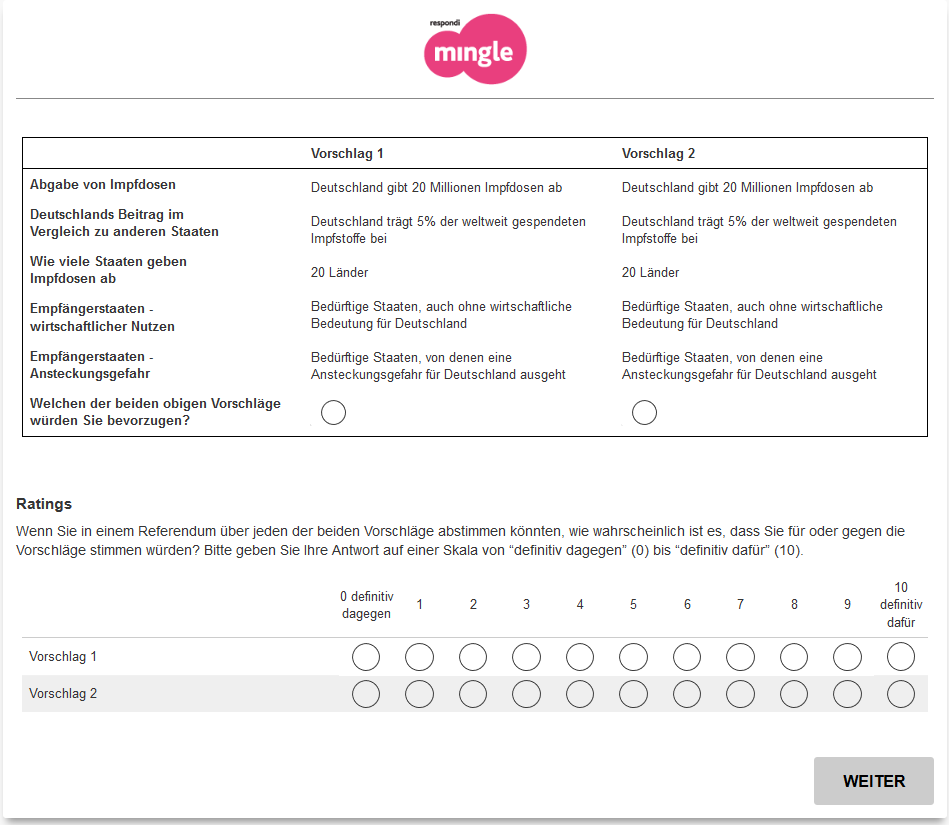
\includegraphics[width=\linewidth]{2_figures/screenshot.png}
\caption{Conjoint Design}
\label{fig:conjoint}

%\floatnote{This is a note for this figure.}
\end{figure}



\newpage
%%%%%%%%%%%%%%%%%%%%%%%%%%




\clearpage
\section{Descriptive Statistics}  

\begin{table}

\caption{\label{tab:SummStats}Summary statistics}
\centering
\resizebox{\linewidth}{!}{
\begin{tabular}[t]{lrrrrrrr}
\toprule
Variable & Mean & Stdev & Minimum & Lower quartile & Median & Upper quartile & Maximum\\
\midrule
Male respondent & 0.49 & 0.50 & 0.0 & 0.00 & 0.00 & 1.00 & 1.00\\
Age (percentile) & 0.47 & 0.28 & 0.0 & 0.21 & 0.47 & 0.70 & 1.00\\
Non German Citizen & 0.03 & 0.16 & 0.0 & 0.00 & 0.00 & 0.00 & 1.00\\
Born outside of Germany & 0.06 & 0.24 & 0.0 & 0.00 & 0.00 & 0.00 & 1.00\\
Migration background of parents & 0.24 & 0.43 & 0.0 & 0.00 & 0.00 & 0.00 & 1.00\\
In former East Germany & 0.15 & 0.36 & 0.0 & 0.00 & 0.00 & 0.00 & 1.00\\
Household size 3 or more & 0.33 & 0.47 & 0.0 & 0.00 & 0.00 & 1.00 & 1.00\\
Employed & 0.43 & 0.50 & 0.0 & 0.00 & 0.00 & 1.00 & 1.00\\
Years of Education & 0.36 & 0.13 & 0.0 & 0.28 & 0.28 & 0.44 & 0.56\\
Voted last elections & 0.82 & 0.38 & 0.0 & 1.00 & 1.00 & 1.00 & 1.00\\
Previously had Covid & 0.04 & 0.18 & 0.0 & 0.00 & 0.00 & 0.00 & 1.00\\
Members of network infected & 0.44 & 0.36 & 0.0 & 0.00 & 0.50 & 0.50 & 1.00\\
Respondent has been vaccinated & 1.77 & 3.23 & 1.0 & 1.00 & 2.00 & 2.00 & 99.00\\
Respondent has been vaccinated & 0.33 & 0.47 & 0.0 & 0.00 & 0.00 & 1.00 & 1.00\\
Believes media exaggerates risk & 0.40 & 0.32 & 0.0 & 0.25 & 0.25 & 0.50 & 1.00\\
Compliance: mask rules & 0.95 & 0.13 & 0.2 & 1.00 & 1.00 & 1.00 & 1.00\\
Compliance: distance rule & 0.90 & 0.17 & 0.2 & 0.80 & 1.00 & 1.00 & 1.00\\
Support distancing even for vaccinated & 0.61 & 0.33 & 0.0 & 0.25 & 0.75 & 1.00 & 1.00\\
Income loss due to Covid (.5 = no change) & 0.57 & 0.19 & 0.0 & 0.50 & 0.50 & 0.75 & 1.00\\
Political interest & 0.67 & 0.28 & 0.0 & 0.67 & 0.67 & 1.00 & 1.00\\
Right leaning & 0.44 & 0.18 & 0.0 & 0.30 & 0.50 & 0.50 & 1.00\\
AfD & 0.08 & 0.27 & 0.0 & 0.00 & 0.00 & 0.00 & 1.00\\
Conservatives & 0.20 & 0.40 & 0.0 & 0.00 & 0.00 & 0.00 & 1.00\\
Liberals & 0.07 & 0.25 & 0.0 & 0.00 & 0.00 & 0.00 & 1.00\\
Green Party & 0.19 & 0.39 & 0.0 & 0.00 & 0.00 & 0.00 & 1.00\\
Left Party & 0.08 & 0.27 & 0.0 & 0.00 & 0.00 & 0.00 & 1.00\\
Social Democrats & 0.13 & 0.33 & 0.0 & 0.00 & 0.00 & 0.00 & 1.00\\
No party identification & 0.22 & 0.42 & 0.0 & 0.00 & 0.00 & 0.00 & 1.00\\
General Trust & 0.43 & 0.27 & 0.0 & 0.20 & 0.50 & 0.60 & 1.00\\
Trust state government & 0.44 & 0.29 & 0.0 & 0.25 & 0.50 & 0.75 & 1.00\\
Trust experts & 0.65 & 0.27 & 0.0 & 0.50 & 0.75 & 0.75 & 1.00\\
Trust federal government & 0.46 & 0.28 & 0.0 & 0.25 & 0.50 & 0.75 & 1.00\\
Trust media & 0.40 & 0.26 & 0.0 & 0.25 & 0.50 & 0.50 & 1.00\\
Trust healthcare & 0.59 & 0.26 & 0.0 & 0.50 & 0.50 & 0.75 & 1.00\\
Values social solidarity & 0.56 & 0.24 & 0.0 & 0.50 & 0.50 & 0.70 & 1.00\\
Values international solidarity & 0.62 & 0.30 & 0.0 & 0.50 & 0.60 & 0.90 & 1.00\\
EU support & 0.52 & 0.30 & 0.0 & 0.30 & 0.50 & 0.70 & 1.00\\
Vaccination Ency & 3.11 & 9.50 & 1.0 & 1.00 & 2.00 & 3.00 & 99.00\\
Migration support & 0.48 & 0.28 & 0.0 & 0.30 & 0.50 & 0.70 & 1.00\\
Covid Protest Contact & 1.66 & 0.47 & 1.0 & 1.00 & 2.00 & 2.00 & 2.00\\
Covid Protest Participation & 1.05 & 0.31 & 1.0 & 1.00 & 1.00 & 1.00 & 4.00\\
Prior Government Performance & -0.83 & 2.75 & -5.0 & -3.00 & -1.00 & 2.00 & 5.00\\
Prior Vaccination Performance & -1.20 & 2.85 & -5.0 & -4.00 & -1.00 & 1.00 & 5.00\\
Prior Vaccination Saliance & 2.09 & 1.11 & 1.0 & 1.00 & 2.00 & 3.00 & 5.00\\
Prior Responsability Government & 8.26 & 2.07 & 0.0 & 7.00 & 9.00 & 10.00 & 10.00\\
Prior Responsability State & 7.09 & 2.46 & 0.0 & 5.00 & 8.00 & 9.00 & 10.00\\
Prior Responsability EU & 6.70 & 2.87 & 0.0 & 5.00 & 7.00 & 9.00 & 10.00\\
Prior Responsability Mayor & 4.79 & 3.02 & 0.0 & 2.00 & 5.00 & 7.00 & 10.00\\
Prior Comparative Performance Germany & 2.60 & 0.63 & 1.0 & 2.00 & 3.00 & 3.00 & 3.00\\
Prior Comparative Performance UK & 1.40 & 0.60 & 1.0 & 1.00 & 1.00 & 2.00 & 3.00\\
Prior Comparative Performance Australia & 2.00 & 0.73 & 1.0 & 1.00 & 2.00 & 3.00 & 3.00\\
Identity Germany & 6.71 & 2.60 & 0.0 & 5.00 & 7.00 & 9.00 & 10.00\\
Identity EU & 5.20 & 2.76 & 0.0 & 3.00 & 5.00 & 7.00 & 10.00\\
Altruism & 6.26 & 2.30 & 0.0 & 5.00 & 6.00 & 8.00 & 10.00\\
Positve Reciprocity & 3.83 & 1.51 & 1.0 & 3.00 & 4.00 & 5.00 & 6.00\\
Negative Reciprocity & 4.88 & 2.74 & 0.0 & 3.00 & 5.00 & 7.00 & 10.00\\
Religiosity & 2.91 & 3.03 & 0.0 & 0.00 & 2.00 & 5.00 & 10.00\\
\bottomrule
\end{tabular}}
\end{table}


%%%%%%%%%%%%%%%%%




\end{document}